\documentclass[titlepage]{article}
\usepackage{amsmath}
\usepackage{epsfig,psfrag}

\setlength{\textwidth}{6.5in}
\setlength{\textheight}{8.9in}
\setlength{\voffset}{-1in}
\setlength{\oddsidemargin}{0in}
\setlength{\evensidemargin}{0in}
\author{Morgan Yost}
\title{Assignment 1}
\begin{document}
\maketitle          
\section{Problem 1}
\subsection{Problem Description}
Let e = (2, -5, 3, 4), find:\\\\
a.$\|e\|_\infty$ b. $\|e\|_1$ c. $\|e\|_2$
\subsection{Problem Solution}
a.\begin{equation*}
\|e\|_\infty = max(|e|) = 5
\end{equation*}
b. \begin{equation*}
\|e\|_1 = \sum_{m=1}^N |e| = 14
\end{equation*}
c. \begin{equation*}
\|e\|_2 = \sqrt{\sum_{m=1}^N e^2} = \sqrt{54}
\end{equation*}

\section{Problem 2}
\subsection{Problem Description}
Let A = \[ \left( \begin{array}{cccc}
1 & 2 & 3 & 4 \\
5 & 6 & 7 & 8 \\
9 & 10 & 11 & 12\\ 
13 & 14 & 15 & 16 \end{array} \right)\] \\
find the following: \\\\
a.$\|A\|_\infty$ b. $\|A\|_1$ c. $\|A\|_2$
\subsection{Problem Solution}
a.\begin{equation*}
\|A\|_\infty = \max_{1\leq i\leq s}\,\sum_{j=1}^s|a_ij| = 58
\end{equation*}
b. \begin{equation*}
\|A\|_1 = \max_{1\leq j\leq s}\,\sum_{i=1}^s|a_ij| = 40
\end{equation*}
c. \begin{equation*}
\|A\|_2 = \sqrt{\rho(A^T A)} = 38.6227
\end{equation*}

\section{Problem 3}
\subsection{Problem Description}
Let $u(x) = x^2-x$, find:
a.$\|u\|_\infty$ b. $\|u\|_1$ c. $\|u\|_2$
\subsection{Problem Solution}
a.\begin{equation*}
\|u\|_\infty = \max_{1\leq 0\leq 1}\,|u| = 1/4
\end{equation*}
\begin{figure}[ht!]
    \centering
    \epsfig{file=3_a.eps}
\end{figure}
b. \begin{equation*}
\|u\|_1 = \int\limits_0^1 |x^2-x| dx = \int{0}^{1} -x^2 -x = \left.\frac{-x^3}{3} + \frac{x^2}{2}\right|_{0}^1 = 1/6
\end{equation*}
c. \begin{equation*}
\|u\|_2 = \sqrt{\int\limits_0^1 |x^2-x|^2 dx} = \sqrt{\int{0}^{1} x^4-2x^3+x^2} = \sqrt{\left.\frac{x^5}{5} - \frac{2x^4}{4} + \frac{x^3}{3}\right|_{0}^1} = \sqrt{-.633}
\end{equation*}
\section{Problem 4}
\subsection{Problem Description}
Let U be defined by $U_i = x_i^1-x_1$ where $x_1 = .2$, $x_2 = .4$, $x_3 = .6$, $x_4 = .8$, $x_5 = 1$. Find the following:
a.$\|U\|_\infty$ b. $\|U\|_1$ c. $\|U\|_2$
\subsection{Problem Solution}
Evaluating $U_i$ for all values of x we find:
U = (-.16, -.24, -.24, -.16, 0). Our grid spacing, h, is .2.
a.\begin{equation*}
\|U\|_\infty = \max_{1\leq 0\leq 1}\,|u| = .24
\end{equation*}
b. \begin{equation*}
\|U\|_1 = h\sum_{m=1}^N |e| = .16
\end{equation*}
c. \begin{equation*}
\|U\|_2 = \sqrt{h\sum_{m=1}^N e^2} = .1824
\end{equation*}

\section{Exercise 1.2}
\subsection{Problem Description}
a. Use method of undetermined coefficients to set up the 5x5 Vandermonde system that would define the fourth-order accurate finite difference approximation to $u^{\prime \prime}(x)$ based on 5 equally spaced points.
\begin{equation*}
u^{\prime \prime}(x) = c_{-2} u(x-2h) + c_{-1} u(x-h) + c_0 u(x) + c_1 u(x+h) + c_2 u(x+2h) + O(h^4)
\end{equation*}
b. Use fdstencil.m to do part a. \\
c. Use this finite difference formula to approximate $u^{\prime \prime}(1)$ for $u(x) = sin(2x)$.
\subsection{Problem Solution}
a. Taylor expansion of the previous equation gives the following:
\begin{equation*}
=u(\bar{x})(c_{-2} + c_{-1} + c_0 + c_1 + c_2) +
\end{equation*}
\begin{equation*}
u^{\prime}(\bar{x})h(-2c_{-2} -c_{-1} +c_1 +2c_2) +
\end{equation*}
\begin{equation*}
u^{\prime \prime}(\bar{x})h^2(2c_{-2} + \frac{1}{2}c_{-1} +\frac{1}{2}c_1 +2c_2) +
\end{equation*}
\begin{equation*}
u^{\prime \prime \prime}(\bar{x})h^3(\frac{-4}{3}c_{-2} - \frac{1}{6}c_{-1} +\frac{1}{6}c_1 + \frac{4}{3}c_2) +
\end{equation*}
\begin{equation*}
u^{\prime \prime \prime \prime}(\bar{x})h^4(\frac{2}{3}c_{-2} +\frac{1}{24}c_{-1} +\frac{1}{24}c_1 +\frac{2}{3}c_2)
\end{equation*}

Choosing to solve for $u^{\prime \prime}(x)$ and putting into matrix form we have: \\
Let A = \[ \left( \begin{array}{ccccc}
1 & 1 & 1 & 1 & 1\\
-2 & -1 & 0 & 1 & 2\\
2 & .5 & 0 & .5 & 2\\
-4/3 & -1/6 & 0 & 1/6 &4/3\\
2/3 & 1/24 & 0 & 1/24 & 2/3 \end{array} \right)\] \\
Let x = \[\left(\begin{array}{c} c_{-2}\\ c_{-1}\\ c_0\\ c_1\\ c_2\end{array}\right)\]
Let b = \[\left(\begin{array}{c} 0\\ 0\\ 1\\ 0\\ 0\end{array}\right)\]
Solving the equation  $Ax=b$, we find that coefficients we are looking for are as follows: \\
x = \[\left(\begin{array}{c} -.0833\\ 1.3333\\ -2.5000\\ 1.3333\\ -.0833\end{array}\right)\]\\
b. Using the fdstencil MATLAB routine resulted in the same answer as seen in part a. The MATALB code is provided in appendix A.\\
c. The errors were calculated in accordance with the equations below:\\
Part A error:
\begin{equation*}
error = |4*sin(2)-B|
\end{equation*}
where B is the result of the estimation scheme used in part A.\\
Part B error:
\begin{equation*}
error = err_0*h^3*u^{\prime \prime \prime \prime \prime} + err_1*h^4*u^{\prime \prime \prime \prime \prime \prime}
\end{equation*}
where $err_0$ and $err_1$ are the coefficients of the 5th and 6th derivatives returned from fdstencil.\\
The comparison for error versus h values is represented by the table below:\\
\begin{center}
\begin{tabular}{ c c c }
 hval & Part A error & Part B error \\ 
0.1000000000000000 & 3.6456044078094720 & 0.000001010330474251 \\ 
0.0562341325190349 & 3.6398506719040853 & 0.000000101033047425 \\ 
0.0316227766016838 & 3.6380311782781858 & 0.000000010103304743 \\ 
0.0177827941003892 & 3.6374558037921250 & 0.000000001010330474 \\ 
0.0100000000000000 & 3.6372738544011982 & 0.000000000101033047 \\ 
0.0056234132519035 & 3.6372163169516960 & 0.000000000010103305 \\ 
0.0031622776601684 & 3.6371981220125749 & 0.000000000001010330 \\ 
0.0017782794100389 & 3.6371923682676237 & 0.000000000000101033 \\ 
0.0010000000000000 & 3.6371905487737117 & 0.000000000000010103 \\ 
0.0005623413251903 & 3.6371899733992166 & 0.000000000000001010 \\ 
0.0003162277660168 & 3.6371897914498255 & 0.000000000000000101 \\ 
0.0001778279410039 & 3.6371897339123755 & 0.000000000000000010 \\ 
0.0001000000000000 & 3.6371897157174367 & 0.000000000000000001 
\end{tabular}
\end{center}

The plots below provide a graphical representation of this data: \\

The trend in both figures shows that the error increases as the h values increase. It makes sense that the estimation scheme would get less accurate as the grid spacing increases. Because the error in part A was calculated by subtracting the actual value from the estimated value, we can see that the truncation error is negligible where the grid spacing is small, then increases drastically as the grid spacing increases. The error calculated by fdstencil shows that the error appears to increase linearly. This is because the error calculation is based on one term, not all of the truncated terms. \\

\begin{figure}[ht!]
    \centering
    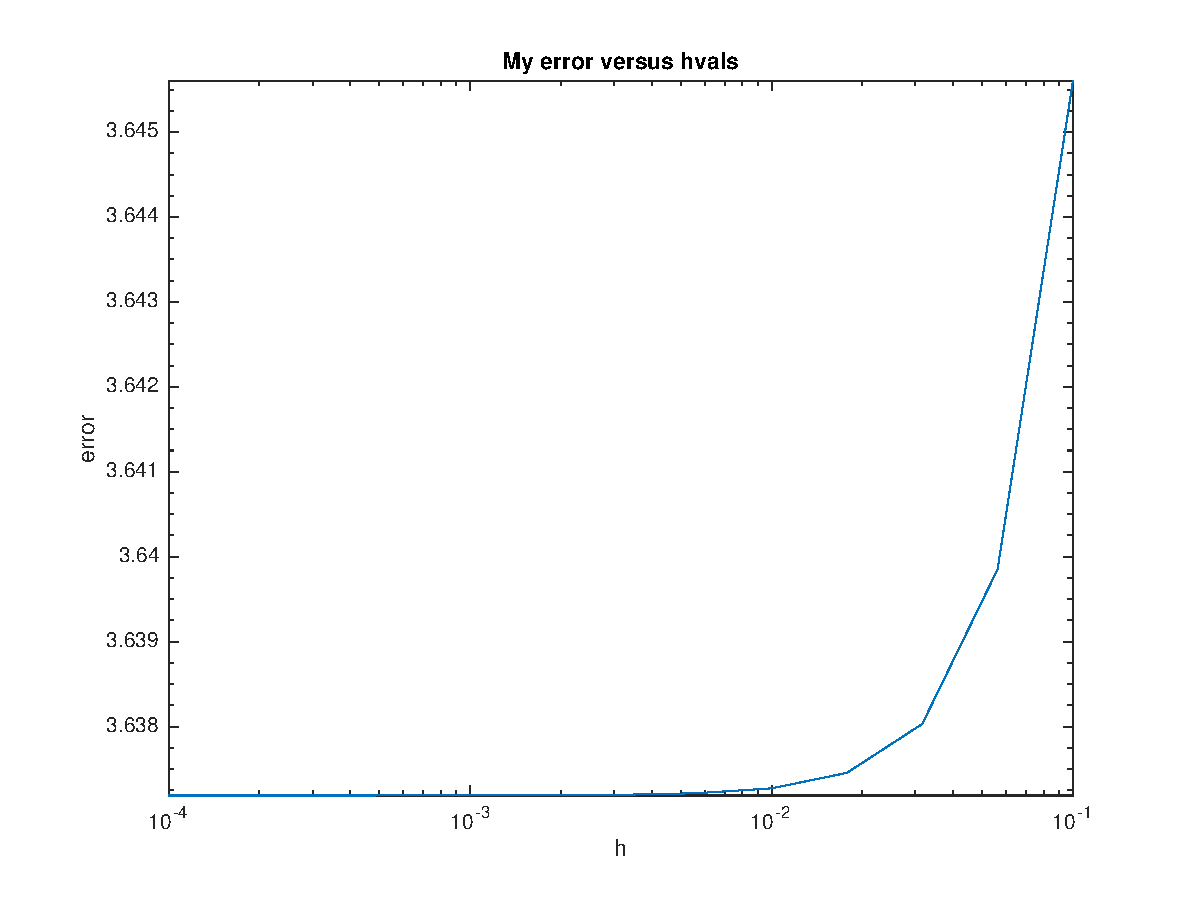
\epsfig{file=my_err.eps}
\end{figure}

\begin{figure}[ht!]
    \centering
    \epsfig{file=fd_err.eps}
\end{figure}

\newpage
\appendix
\section{MATLAB Code}
\end{document}
